%%%%%%%%%%%%%%%%%%%%%%%%%%%%% Define Article %%%%%%%%%%%%%%%%%%%%%%%%%%%%%%%%%%
\documentclass{article}
%%%%%%%%%%%%%%%%%%%%%%%%%%%%%%%%%%%%%%%%%%%%%%%%%%%%%%%%%%%%%%%%%%%%%%%%%%%%%%%

%%%%%%%%%%%%%%%%%%%%%%%%%%%%% Using Packages %%%%%%%%%%%%%%%%%%%%%%%%%%%%%%%%%%
\usepackage{graphicx}
\usepackage[margin=1in]{geometry}
\usepackage{amssymb}
\usepackage{amsmath}
\usepackage{amsthm}
\usepackage{empheq}
\usepackage{mdframed}
\usepackage{booktabs}
\usepackage{indentfirst}
\usepackage{lipsum}
\usepackage{graphicx}
\usepackage{color}
\usepackage{psfrag}
\usepackage{pgfplots}
\usepackage{bm}
\usepackage{listings}
\usepackage{xcolor}
%%%%%%%%%%%%%%%%%%%%%%%%%%%%%%%%%%%%%%%%%%%%%%%%%%%%%%%%%%%%%%%%%%%%%%%%%%%%%%%

% Other Settings

%%%%%%%%%%%%%%%%%%%%%%%%%% Page Setting %%%%%%%%%%%%%%%%%%%%%%%%%%%%%%%%%%%%%%%
\geometry{a4paper}

%%%%%%%%%%%%%%%%%%%%%%%%%% Define some useful colors %%%%%%%%%%%%%%%%%%%%%%%%%%
\definecolor{ocre}{RGB}{243,102,25}
\definecolor{mygray}{RGB}{243,243,244}
\definecolor{deepGreen}{RGB}{26,111,0}
\definecolor{shallowGreen}{RGB}{235,255,255}
\definecolor{deepBlue}{RGB}{61,124,222}
\definecolor{shallowBlue}{RGB}{235,249,255}
%%%%%%%%%%%%%%%%%%%%%%%%%%%%%%%%%%%%%%%%%%%%%%%%%%%%%%%%%%%%%%%%%%%%%%%%%%%%%%%
\definecolor{codegreen}{rgb}{0,0.6,0}
\definecolor{codegray}{rgb}{0.5,0.5,0.5}
\definecolor{codepurple}{rgb}{0.58,0,0.82}
\definecolor{backcolour}{rgb}{0.95,0.95,0.92}

\lstdefinestyle{mystyle}{
    backgroundcolor=\color{backcolour},   
    commentstyle=\color{codegreen},
    keywordstyle=\color{magenta},
    numberstyle=\tiny\color{codegray},
    stringstyle=\color{codepurple},
    basicstyle=\ttfamily\footnotesize,
    breakatwhitespace=false,         
    breaklines=true,                 
    captionpos=b,                    
    keepspaces=true,                 
    numbers=left,                    
    numbersep=5pt,                  
    showspaces=false,                
    showstringspaces=false,
    showtabs=false,                  
    tabsize=2
}

\lstset{style=mystyle}
%%%%%%%%%%%%%%%%%%%%%%%%%% Define an orangebox command %%%%%%%%%%%%%%%%%%%%%%%%
\newcommand\orangebox[1]{\fcolorbox{ocre}{mygray}{\hspace{1em}#1\hspace{1em}}}
%%%%%%%%%%%%%%%%%%%%%%%%%%%%%%%%%%%%%%%%%%%%%%%%%%%%%%%%%%%%%%%%%%%%%%%%%%%%%%%

%%%%%%%%%%%%%%%%%%%%%%%%%%%% English Environments %%%%%%%%%%%%%%%%%%%%%%%%%%%%%
\newtheoremstyle{mytheoremstyle}{3pt}{3pt}{\normalfont}{0cm}{\rmfamily\bfseries}{}{1em}{{\color{black}\thmname{#1}~\thmnumber{#2}}\thmnote{\,--\,#3}}
\newtheoremstyle{myproblemstyle}{3pt}{3pt}{\normalfont}{0cm}{\rmfamily\bfseries}{}{1em}{{\color{black}\thmname{#1}~\thmnumber{#2}}\thmnote{\,--\,#3}}
\theoremstyle{mytheoremstyle}
\newmdtheoremenv[linewidth=1pt,backgroundcolor=shallowGreen,linecolor=deepGreen,leftmargin=0pt,innerleftmargin=20pt,innerrightmargin=20pt,]{theorem}{Theorem}[section]
\theoremstyle{mytheoremstyle}
\newmdtheoremenv[linewidth=1pt,backgroundcolor=shallowBlue,linecolor=deepBlue,leftmargin=0pt,innerleftmargin=20pt,innerrightmargin=20pt,]{definition}{Definition}[section]
\theoremstyle{myproblemstyle}
\newmdtheoremenv[linecolor=black,leftmargin=0pt,innerleftmargin=10pt,innerrightmargin=10pt,]{problem}{Problem}[section]
%%%%%%%%%%%%%%%%%%%%%%%%%%%%%%%%%%%%%%%%%%%%%%%%%%%%%%%%%%%%%%%%%%%%%%%%%%%%%%%

%%%%%%%%%%%%%%%%%%%%%%%%%%%%%%% Plotting Settings %%%%%%%%%%%%%%%%%%%%%%%%%%%%%
\usepgfplotslibrary{colorbrewer}
\pgfplotsset{width=8cm,compat=1.9}
%%%%%%%%%%%%%%%%%%%%%%%%%%%%%%%%%%%%%%%%%%%%%%%%%%%%%%%%%%%%%%%%%%%%%%%%%%%%%%%

%%%%%%%%%%%%%%%%%%%%%%%%%%%%%%% Title & Author %%%%%%%%%%%%%%%%%%%%%%%%%%%%%%%%
\title{\textbf{BANA 620 PROJECT REPORT: DESCRIPTIVE AND PREDICTIVE ANALYTICS APPLIED TO THE SKILLED NURSING FACILITY COST REPORTS}}
\author{Joshua Cabal \\ \\ \\California State University, Northridge \\}
%%%%%%%%%%%%%%%%%%%%%%%%%%%%%%%%%%%%%%%%%%%%%%%%%%%%%%%%%%%%%%%%%%%%%%%%%%%%%%%

\begin{document}
    \maketitle
    \pagebreak
    \tableofcontents    
    \newpage


%-------------------BEGIN: Executive Summary------------------------------------
\section{Executive Summary}

An overview of the project, including key findings, recommendations, and a brief summary of the analysis conducted. This section should be concise and geared toward readers who may not delve into the full details of the report. 

%-------------------END: Executive Summary------------------------------------
%-------------------BEGIN: Introduction------------------------------------
\section{Introduction}

Context and background information about the opportunity the project addresses. This section should outline the objectives of the project and the significance of the analysis being conducted.
%-------------------END: Introduction------------------------------------
%-------------------BEGIN: Methodology------------------------------------
\section{Methodology}
A detailed description of the analytical methods and tools used in the project. This should include data collection processes, data analysis techniques (e.g., statistical methods, machine learning algorithms), and any software or programming languages utilized.



%-------------------END: Methodology------------------------------------
%-------------------BEGIN: Data Description------------------------------------
\section{Data Description}

An overview of the data set(s) used, including sources, size, and characteristics of the data. Highlight any data cleaning or preprocessing steps undertaken to prepare the data for analysis.



\subsection{Skilled Nusing Facility Cost Report}

Medicare-certified institutional providers are required to submit annual cost reports. These data files contain the highest level of cost report status for cost reports in each reported fiscal years. The cost report contains provider information such as facility characteristics, utilization data, cost and charges by cost center (in total and for Medicare), Medicare settlement data, and financial statement data. CMS maintains the cost report data in the Healthcare Provider Cost Reporting Information System (HCRIS). Skilled Nursing Facilities (SNF) submit their cost report data to HCRIS using form CMS-2540-2010. The reports used are from the years 2015 through 2021.

\subsubsection{Preprocessing: Data Loading and Handling Missing Values}
Since each year has their own .csv file, the several skilled nursing facility cost reports needed to be concatenated into a single DataFrame. In order to do this, the headers fom years 2020 and 2021 had to be made consistent with the headers from the other years. This was manually completed in Microsoft Excel, and the similar columns were renamed accordingly. Any columns that were unable to be matched were dropped and a Year attribute was added to all records during the import step. Finally, the headers were changed to only lowercase for consistency. 

After import, the next step was to handle the null values. I began with column leveling cleaning and defined two different lists which contain the columns that will be dropped: dropNull, dropRedundancy. As the list names demonstrate, these attributes will only hinder model performance, if incldued. The first list, dropNull, contains the columns which contain an overwhelming majority, over 90\%, of null values across all records. The second list, dropRedundancy, contains the columns which contain data that are captured within other attributers. Because the submitted financial form requires as breakdown of some of the reported numbers, these columns were removed and only the highest level feature was kept.  

To handle the remaining null values, I proceeded with record level cleaning by simple imputation. In this case, I used mean imputation and rounded to the nearest integer. I rounded to the nearest integer because a few of the attributes attain values only belonging to the integers. After all loading, 55 columns remained from the initial 100. 


\subsubsection{Preprocessing: Handling Outliers}
The first method used to handle outliers was by z-score threshold. As the name implies, this method works by choosing a z-score threshold and removing all records which attain values outside this window. In my case, I used the value of 3 as my threshold and chose the target columns net income and accounts payable. These values were chosen because, after testing against multiple different attributes and with varying thresholds, using these as the target columns handled many of the outliers. 

\begin{lstlisting}[language=Python, caption=Function to clean by z-score threshold]
# dealing with a subset of outliers by z-score threshold
def removeOutliers(input_df, column_name, zScoreThreshold):
    mean = input_df[column_name].mean()
    std = input_df[column_name].std()
    z_scores = (input_df[column_name] - mean) / std

    return input_df[(z_scores > -zScoreThreshold) & (z_scores < zScoreThreshold)]

numerical_columns = ['net_income', 'accounts_payable']
for each in numerical_columns:
   df = removeOutliers(fullCostReportdf, each, 3)
\end{lstlisting}

After this was completed, the data was manually brushed through for more outliers and the only attribute which contained suspect outliers to be removed was the number of beds. Eleven nursing facilities had reported having over 21000 beds, and therefore, we defined a variable named bedThreshold and removed all the records which had more than this threshold. 
%-------------------END: Data Description------------------------------------
%-------------------BEGIN: Analysis and Findings------------------------------------
\section{Analysis and Findings}

Presentation of the analysis conducted, including data visualization (charts, graphs, tables) and statistical outputs. This section should detail the insights gained from the analysis, interpreting the results in the context of the business problem.
%-------------------END: Analysis and Findings------------------------------------
%-------------------BEGIN: Discussion------------------------------------
\section{Discussion}
Interpretation of the findings, discussing how they address the project objectives and their implications for the business. This section should also cover any limitations of the analysis and considerations for future research.

%-------------------END: Discussion------------------------------------
%-------------------BEGIN: Recommendations------------------------------------
\section{Recommendations}
Based on the analysis and findings, provide actionable recommendations for the business. Clearly articulate the expected impact of these recommendations and suggest a plan for implementation.

%-------------------END: Recommendations------------------------------------
%-------------------BEGIN: Conclusion------------------------------------
\section{Conclusion}
Summarize the key points from the report, reinforcing the value of the findings and recommendations.

%-------------------END: Conclusion------------------------------------
%-------------------BEGIN: Appendices------------------------------------
\section{Appendices}
Include any additional material that supports the analysis, such as detailed data tables, code snippets, or extended methodology descriptions.

\begin{figure}[htbp]
\centering
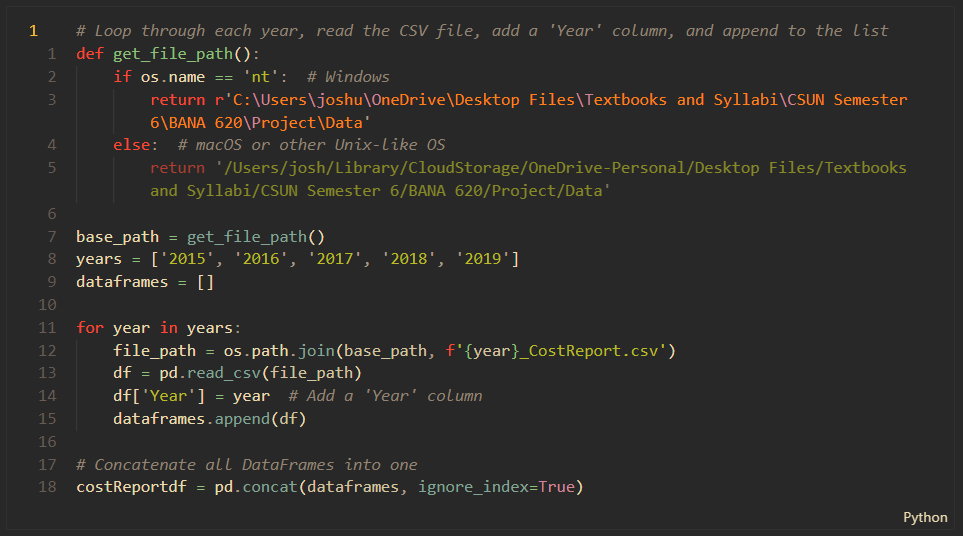
\includegraphics[width=\linewidth]{./Images/dataLoadingSnippet.png}
\caption{Data loading code snippet}
\label{fig:screenshot_label}
\end{figure}

%-------------------END: Appendices------------------------------------

%-------------------BEGIN: References------------------------------------
\section{References}
List all sources cited in the report, including data sources, literature, and any external references used in the analysis.

%-------------------END: References------------------------------------



\end{document}